\section{STT-RAM Macro Design Optimization} \label{sec:opt}
In this section we first choose two MTJ specs as our optimization targets. After numerous simulations we the importance of careful write pulse width selection is revealed for optimizing area, read latency/energy, write latency/enery and leakage power of STT-RAM. Then we will focus on the analysis of write energy optimization, which is both device and capacity dependent. Finally we will combine the improved architectural design together with the write pulse width optimization to illustrate a full design explore a STT-RAM chip.

\subsection{Impact of Write Pulse Width}
As discussed in Section~\ref{subsec:ict}, a wide range of coupled switching current and switching time can be operated for STT-RAM cell. In this work, we will focus on processional switching mode and dynamic reversal mode, particularly, for $0.4ns < \tau < 10ns$. We choose two curves which can represent the typical switching characteristics of in-plane MTJ~\cite{STTRAM:Qualcomm09} and PMTJ~\cite{PMTJ:Toshiba08}. As seen in Figure~{fig:specs}, PMTJ has remarkable advantages over in-plane MTJ in both switching current and switching energy for any given write pulse width assuming the same ratio of damping constant to STT efficiency. We also assume the same TMR and resistance for in-plane MTJ and PMTJ. For PMTJ, realization of matching these parameters of in-plane MTJ needs some device-level efforts as mentioned in Section~\ref{subsec:pmtj}.

\begin{comment}
Short write pulse induced large switching current requires large access transistor for providing enough driving current, which consequently brings more circuit design challenges of the STT-RAM prototype. Particularly, the gate of the access device is connected to the wordline and its drain is connected to bitline. When larger MOS transistor is in serial, the increased gate and drain capacitance will contribute to wordline capacitance and bitline capacitance, which means increased wordline/bitline RC delay and dynamic energy. What��s more, larger selection device
consumes more area. Components of peripheral circuit such as decoder buffer size, determined by the load capacitance, also increase, which results in larger area, longer RC delay and more dynamic energy consumption.
\end{comment} 

\begin{figure}[t]
  \centering
  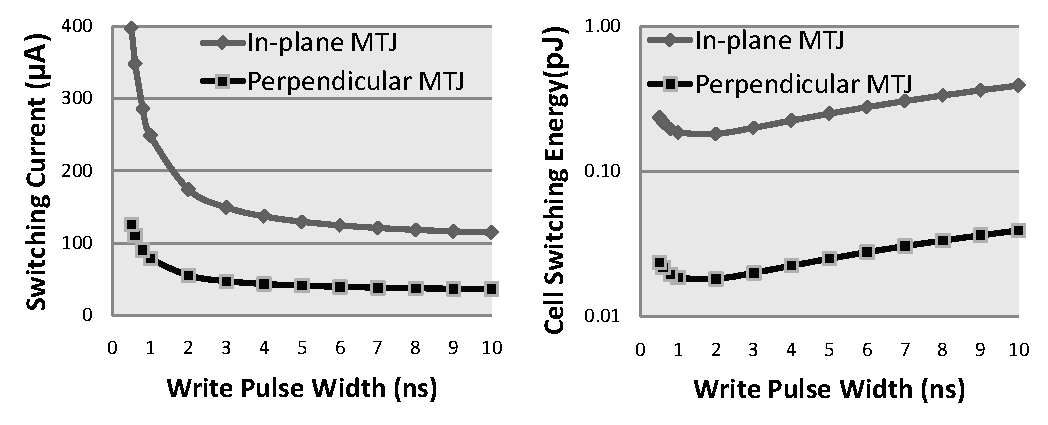
\includegraphics[width=3.5in]{fig/MTJSpec.eps}
  \caption{Representative data curves of in-plane and perpendicular MTJs: (a)Switching current; (b) Cell switching energy.}
  \label{fig:specs}
\end{figure}

\begin{figure*}[t]
  \centering
  \includegraphics[width=7in]{fig/AllMetrics.eps}
  \caption{Metrics of SRAM and STT-RAM built with in-plane and perpendicular MTJs: (a)Area; (b)Read latency; (c)Read energy; (d)Write latency; (e)Write energy; (f)Leakage power.}
  \label{fig:metrics}
\end{figure*}

\subsection{Write Energy Optimization}

\begin{comment}
It is also observed that optimal setting of write time for STT-RAM is function of capacity. Given a fixed word length, the proportion of dynamic energy consumption on memory cells decreases as capacity increases. Energy on peripheral circuitry begins to decimate at large memory capacity. Thus the energy consumption on memory cells and peripheral circuitry goes in opposite directions and the optimal write pulse width increase with capacity increase.
\end{comment} 

\begin{figure}[t]
  \centering
  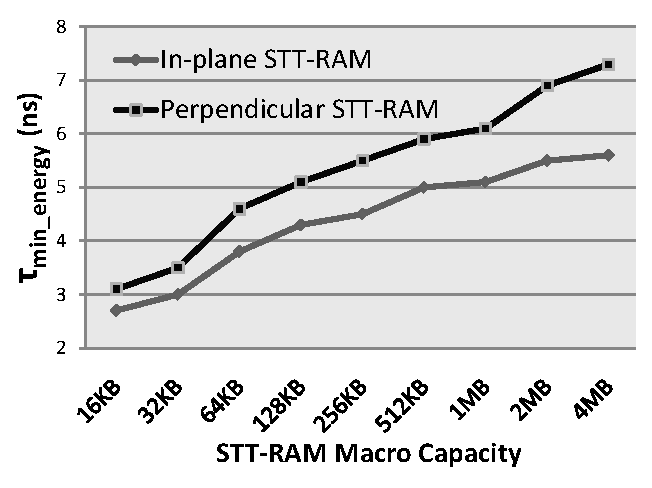
\includegraphics[width=3in]{fig/MinEnergy.eps}
  \caption{Dependence of $\tau_{min\_energy}$ on STT-RAM Macro Capacity.}
  \label{fig:minenergy}
\end{figure}

\subsection{Device-Architecture Co-Optimization}

\begin{table*}[t]
%\vspace{-5pt}
\centering
\caption{Device-Architecture Co-Optimization of a 45nm 64MB STT-RAM chip}
\label{tb:bigtable}
%\vspace{-5pt}
\begin{tabular}{| l | c | c | c | c | c | c |}
\hline\hline
& Area opt. & Read latency opt. & Write latency opt. & Read energy opt. & Write energy opt. & Leakage opt. \\
\hline
Area ($mm^2$) & \textbf{3.06} & 10.7 & 16.4 & 5.66 & 6.22 & 3.63 \\
\hline
Read latency ($ns$) & 21.8 & \textbf{3.70} & 4.92 & 9.12 & 9.57 &	9.91 \\
\hline
Write latency ($ns$) & 18.6	& 13.9	& \textbf{4.0}1	& 15.9	& 12.3	& 18.1 \\
\hline
Read energy ($nJ$) & 0.276	& 0.225	& 0.316	& \textbf{0.105}	& 0.139	& 0.279 \\
\hline
Write energy ($nJ$) & 0.293	& 0.322	& 0.309	& 0.193	& \textbf{0.131}	& 0.281\\
\hline
Leakage ($W$) & 1.01	& 3.53	& 4.98	& 1.85	& 1.92	& \textbf{0.78}\\
\hline\hline
Write pulse width ($ns$) & 10 & 10 & 2 & 10 & 6 & 10 \\
\hline
Inter-array routing & Non-H-tree & H-tree & H-tree & H-tree & H-tree & Non-H-tree \\
\hline
Sense amp placement & External & Internal & Internal & Internal & Internal & External \\
\hline
Sense amp type & Current-in voltage & Current & Current & Voltage-divider & Voltage-divider & Voltage-divider \\
\hline
Interconnect wire & Normal & Repeated & Repeated & Low-swing & Low-swing & Normal \\
\hline
Output buffer type & Area opt. & Latency opt. & Latency opt. & Area opt. & Area opt. & Area opt. \\
\hline\hline
\end{tabular}
%\vspace{-10pt}
\end{table*} 